%% ==========================================================================
%%  dgnozzle -- logical grid to physical nozzle mapping
%% ==========================================================================
\ifdefined\DGNOZZLEEMBEDDED\else
\documentclass[tikz,border=6pt]{standalone}
\usepackage{amsmath}
\usetikzlibrary{arrows.meta,calc}
\begin{document}
\fi

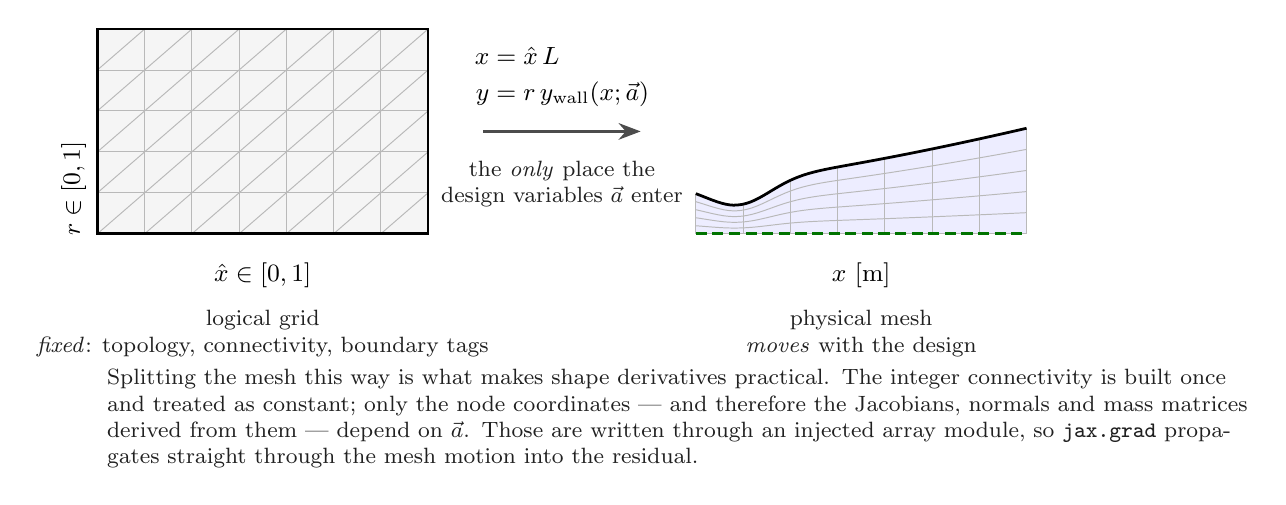
\begin{tikzpicture}[
  >={Stealth[length=2.8mm]},
  grid/.style = {gray!55, line width=0.35pt},
  bd/.style   = {line width=1.0pt},
  lbl/.style  = {font=\small},
  slbl/.style = {font=\footnotesize, gray!25!black},
]

%% ---- logical square ------------------------------------------------------
\begin{scope}
  \fill[black!4] (0,0) rectangle (4.2,2.6);
  \foreach \i in {0,...,7} \draw[grid] (\i*0.6,0) -- (\i*0.6,2.6);
  \foreach \j in {0,...,5} \draw[grid] (0,\j*0.52) -- (4.2,\j*0.52);
  \foreach \i in {0,...,6} \foreach \j in {0,...,4}
    \draw[grid] (\i*0.6,\j*0.52) -- (\i*0.6+0.6,\j*0.52+0.52);
  \draw[bd] (0,0) rectangle (4.2,2.6);
  \node[lbl, anchor=north] at (2.1,-0.25) {$\hat{x} \in [0,1]$};
  \node[lbl, anchor=east, rotate=90] at (-0.3,1.3) {$r \in [0,1]$};
  \node[slbl, anchor=north, align=center] at (2.1,-0.85)
    {logical grid\\ \emph{fixed}: topology, connectivity, boundary tags};
\end{scope}

%% ---- the map -------------------------------------------------------------
\draw[->, line width=1.2pt, black!70] (4.9,1.3) -- (6.9,1.3);
\node[lbl, anchor=south, align=center] at (5.9,1.45)
  {$\displaystyle \begin{aligned} x &= \hat{x}\,L\\[-1pt]
    y &= r\, y_{\mathrm{wall}}(x;\vec{a})\end{aligned}$};
\node[slbl, anchor=north, align=center, text width=3.4cm] at (5.9,1.05)
  {the \emph{only} place the design variables $\vec{a}$ enter};

%% ---- physical nozzle -----------------------------------------------------
\begin{scope}[xshift=7.6cm]
  \def\wall#1{0.62 + 1.05*(#1)*(#1) - 0.22*(#1)}
  \fill[blue!7] plot[domain=0:4.2,samples=60]
        (\x, {0.62 - 0.30*exp(-((\x-0.55)/0.55)^2) + 0.30*(\x/4.2)^1.35*2.4})
        -- (4.2,0) -- (0,0) -- cycle;
  \foreach \j in {0,...,5}
    \draw[grid] plot[domain=0:4.2,samples=60]
      (\x, {(\j/5)*(0.62 - 0.30*exp(-((\x-0.55)/0.55)^2) + 0.30*(\x/4.2)^1.35*2.4)});
  \foreach \i in {0,...,7}
    \draw[grid] (\i*0.6,0) --
      (\i*0.6, {0.62 - 0.30*exp(-((\i*0.6-0.55)/0.55)^2) + 0.30*(\i*0.6/4.2)^1.35*2.4});
  \draw[bd] plot[domain=0:4.2,samples=80]
      (\x, {0.62 - 0.30*exp(-((\x-0.55)/0.55)^2) + 0.30*(\x/4.2)^1.35*2.4});
  \draw[bd, green!45!black, dash pattern=on 4pt off 2pt] (0,0) -- (4.2,0);
  \node[lbl, anchor=north] at (2.1,-0.25) {$x$ [m]};
  \node[slbl, anchor=north, align=center] at (2.1,-0.85)
    {physical mesh\\ \emph{moves} with the design};
\end{scope}

\node[slbl, align=left, anchor=north west, text width=14.5cm] at (0,-1.6)
  {Splitting the mesh this way is what makes shape derivatives practical.  The
   integer connectivity is built once and treated as constant; only the node
   coordinates --- and therefore the Jacobians, normals and mass matrices
   derived from them --- depend on $\vec{a}$.  Those are written through an
   injected array module, so \texttt{jax.grad} propagates straight through the
   mesh motion into the residual.};

\end{tikzpicture}

\ifdefined\DGNOZZLEEMBEDDED\else
\end{document}
\fi
